\chapter{Algorithm and Implementation}
In this chapter, we'll look into the algorithm overview and the corresponding code implementation.

\section{Pre-Computing Optical Depth}
The first step is to pre-compute the optical depth using Equation 2.2: $\tau(A, B) = \int_{A}^{B}\beta(P)\cdot ds$ for each ray to the boundary of a certain particle. The author assumed that the camera will always stay outside the volume. Then, the goal of this step is to calculate the optical depth integral for all possible camera positions and orientations.

\begin{figure}[htp]
\begin{center}
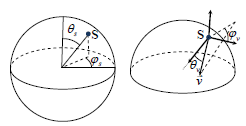
\includegraphics[scale=1.0]{images/startandview.png}
\caption{Four angels to describe a ray}
\label{f8}
\end{center}
\end{figure}

\subsection{The Design}
To describe a ray, we need 4 angles, 2 angles describing the start point on the particle sphere, and 2 angles describing the view direction. Because of the 4 parameters, a 4D look-up table is necessary. As shown in the figure above, $\varphi_S\in[0, 2\pi]$ and $\theta_S\in[0, \pi]$ are used to specify the start point of the ray. While $\varphi_v\in[0, 2\pi]$ and $\theta_v\in[0, \frac{\pi}{2}]$ are used to specify the direction of the ray.\\\\\\

\begin{figure}[htp]
\begin{center}
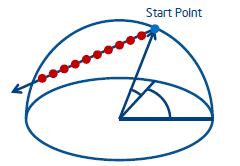
\includegraphics[scale=0.5]{images/opticaldepthintegration.png}
\caption{Numerically integrate the optical depth of a ray}
\label{f9}
\end{center}
\end{figure}

Then we use Equation 2.2: $\tau(A, B) = \int_{A}^{B}\beta(P)\cdot ds$ to accumulate the optical depth of a ray. Now, here is the interesting part of how to retrieve the extinction coefficient $\beta(P)$. The author used 4D look-tables which contains several 3D noises to get the extinction coefficient. The figure below shows one typical noise texture.

\begin{figure}[htp]
\begin{center}
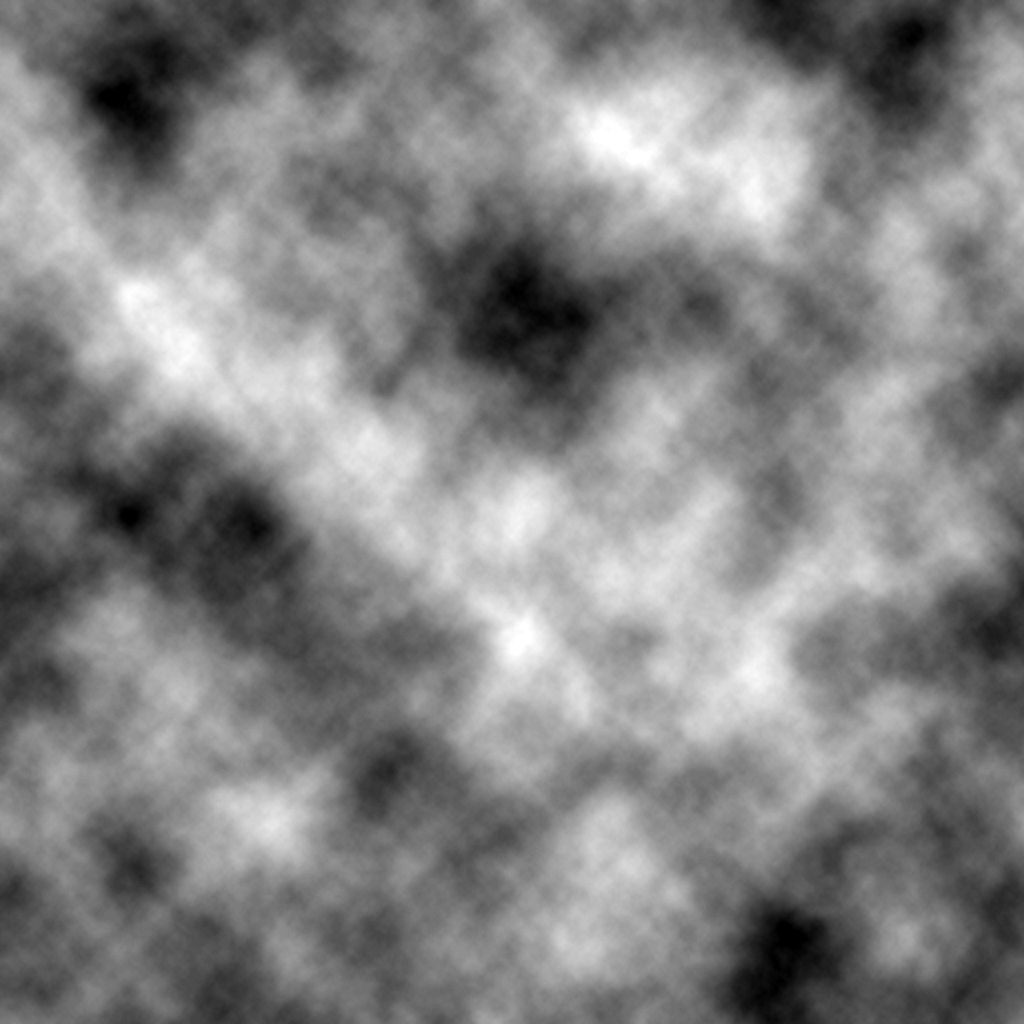
\includegraphics[scale=0.1]{images/Noise.png}
\caption{A typical noise texture}
\label{f10}
\end{center}
\end{figure}

\subsection{The Implementation}
After carefully explaining the design of the first step, let's have a look at how the actual related function in the shader looks like. Please note that the rendering API is \textbf{DirectX}, hence the shader is written in \textbf{HLSL}.\\\\
\begin{lstlisting}
// This shader computes level 0 of the maximum density mip map
float2 PrecomputeOpticalDepthPS(SScreenSizeQuadVSOutput In) : SV_Target
{
    float3 f3NormalizedStartPos, f3RayDir;
    OpticalDepthLUTCoordsToWorldParams( float4(ProjToUV(In.m_f2PosPS), g_GlobalCloudAttribs.f4Parameter.xy), f3NormalizedStartPos, f3RayDir );
    
    // Intersect view ray with the unit sphere:
    float2 f2RayIsecs;
    // f3NormalizedStartPos  is located exactly on the surface; slightly move start pos inside the sphere
    // to avoid precision issues
    GetRaySphereIntersection(f3NormalizedStartPos + f3RayDir*1e-4, f3RayDir, 0, 1.f, f2RayIsecs);
    
    if( f2RayIsecs.x > f2RayIsecs.y )
        return 0;

    float3 f3EndPos = f3NormalizedStartPos + f3RayDir * f2RayIsecs.y;
    float fNumSteps = NUM_INTEGRATION_STEPS;
    float3 f3Step = (f3EndPos - f3NormalizedStartPos) / fNumSteps;
    float fTotalDensity = 0;
    float fDistToFirstMatter = -1;
    for(float fStepNum=0.5; fStepNum < fNumSteps; ++fStepNum)
    {
        float3 f3CurrPos = f3NormalizedStartPos + f3Step * fStepNum;
        
        float fDistToCenter = length(f3CurrPos);
        float fMetabolDensity = GetMetabolDensity(fDistToCenter);
        float fDensity = 1;
#if DENSITY_GENERATION_METHOD == 0
        fDensity = saturate( 1.0*saturate(fMetabolDensity) + 1*pow(fMetabolDensity,0.5)*(GetRandomDensity(f3CurrPos, 0.15, 4, 0.7 )) );
#elif DENSITY_GENERATION_METHOD == 1
        fDensity = 1.0*saturate(fMetabolDensity) + 1.0*pow(fMetabolDensity,0.5)*(GetRandomDensity(f3CurrPos, 0.1,4,0.8)) > 0.1 ? 1 : 0;
#elif DENSITY_GENERATION_METHOD == 2
        fDensity = GetPyroSphereDensity(f3CurrPos);
#endif

        if( fDensity > 0.05 && fDistToFirstMatter < 0 )
            fDistToFirstMatter = fStepNum / fNumSteps;
       
        fTotalDensity += fDensity;
    }
    if( fDistToFirstMatter < 0 ) fDistToFirstMatter = 1;
    return float2(fTotalDensity / fNumSteps, fDistToFirstMatter);
}
\end{lstlisting}


The integration function is \textbf{PrecomputeOpticalDepthPS}. Firstly, it decomposes the given projection position and the 4 angle parameters from inhomogeneous coordinates into 2 vec3 positions, the first one \textbf{f3NormalizedStartPos} describes the start position of the ray, the second one \textbf{f3RayDir} describes the ray direction. Then the intersecting view ray inside the unit sphere is calculated. Since the start position is just on the surface of the sphere, in order to avoid precision issues, the author moved the start position slightly into the sphere by the amount of \textbf{f3RayDir*1e-4}. Then the integration is done inside the \textbf{for loop}. \textbf{DENSITY\_GENERATION\_METHOD} is defined as: 0 represents radial fall-off + 3D noise, 1 represents 3D noise + thresholding, 2 represents pyroclastic style.
\textbf{fDensity} is the current density of this step. Finally, the total density \textbf{fTotalDensity} for a ray is accumulated.


\section{Pre-Computing Scattering}
In this step, the author proposed with two types of scattering: single scattering and multiple scattering. In nature, a photon inside a cloud is scattered multiple times before it leaves the cloud. Hence the author concentrated on the multiple scattering in order to render a realistic cloud appearance. The goal is to calculate multiple scattering for every possible light position, camera position and orientation.

\subsection{Single Scattering}
\subsubsection{The Design}
\begin{figure}[htp]
\begin{center}
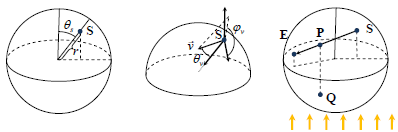
\includegraphics[scale=1.0]{images/singlescattering.png}
\caption{Pre-computing single scattering inside the spherical
particle}
\label{f11}
\end{center}
\end{figure}
First of all, the author assumed that the particle density only depends on the distance to the center. As the particle is a perfect sphere, which has the nature of symmetry, the author indicated that an arbitrary light direction coinciding with positive $z$ axis can be chosen to examine one of the rays that intersect the sphere. Since the light field is also symmetrical, only one angle $\theta_S$ is needed to describe the start point of a ray. As discussed in the previous section, another 2 angles $\phi_v$ and $\theta_v$ will still be needed to describe the ray direction. As the light field inside the volumes is important to solve the scattering equation, the author introduced a 4D look-up table with 3 angles($\theta_S$, $\phi_v$ and $\theta_v$) and the fraction of distance $r$ from the center of the sphere. We note the table as 
\begin{equation}
\bar{L}^{(1)}_{In}(\theta_S, \phi_v, \theta_v, r), \theta_S\in[0, \pi], \phi_v\in[0, \pi], \theta_v\in[0, \pi], r\in[0, 1].
\end{equation}
The author then proposed with a solution to single scattering inside the spherical particle:
\begin{equation}
\bar{L}^{(1)}_{In} = \int_{S}^{E}e^{-\tau(P,S)}e^{-\tau(P,Q)} \cdot \beta(P) \cdot ds,
\end{equation}
where \textbf{S} is the start point of the ray and \textbf{E} is the exit point of the ray. \textbf{Q} is the point on the surface of the sphere through which the light reaches the current integration point \textbf{P}. The author finally implied that the phase function $P(\theta)$ is only used at run time to avoid precision issues. Just like the optical depth calculation, the extinction coefficient $\beta(P)$ can be evaluated in different methods as long as the distance to the center is the only influencing factor. The author tried different methods and finally decided to make the density constant.

\subsubsection{The Implementation}
Let's have a look at the implementation detail in code.
\begin{lstlisting}
float PrecomputeSingleSctrPS(SScreenSizeQuadVSOutput In) : SV_Target
{
    float4 f4LUTCoords = float4(ProjToUV(In.m_f2PosPS), g_GlobalCloudAttribs.f4Parameter.xy);
    float3 f3EntryPointUSSpace, f3ViewRayUSSpace, f3LightDirUSSpace;
    float fDensityScale;
    ParticleScatteringLUTToWorldParams(f4LUTCoords, g_GlobalCloudAttribs.f4Parameter.z, f3EntryPointUSSpace, f3ViewRayUSSpace, f3LightDirUSSpace, false, fDensityScale);
    // Intersect view ray with the unit sphere:
    float2 f2RayIsecs;
    // f3NormalizedStartPos  is located exactly on the surface; slightly move the start pos inside the sphere
    // to avoid precision issues
    float3 f3BiasedEntryPoint = f3EntryPointUSSpace + f3ViewRayUSSpace*1e-4;
    GetRaySphereIntersection(f3BiasedEntryPoint, f3ViewRayUSSpace, 0, 1.f, f2RayIsecs);
    if( f2RayIsecs.y < f2RayIsecs.x ) return 0;
    float3 f3EndPos = f3BiasedEntryPoint + f3ViewRayUSSpace * f2RayIsecs.y;
    float fNumSteps = NUM_INTEGRATION_STEPS;
    float3 f3Step = (f3EndPos - f3EntryPointUSSpace) / fNumSteps;
    float fStepLen = length(f3Step);
    float fCloudMassToCamera = 0;
    float fParticleRadius = GetParticleSize(GetCloudRingWorldStep(0, g_GlobalCloudAttribs));
    float fInscattering = 0;
    for(float fStepNum=0.5; fStepNum < fNumSteps; ++fStepNum)
    {
        float3 f3CurrPos = f3EntryPointUSSpace + f3Step * fStepNum;
        float fDensity = 1;
        fDensity *= fDensityScale;
        float fCloudMassToLight = 0;
        GetRaySphereIntersection(f3CurrPos, f3LightDirUSSpace, 0, 1.f, f2RayIsecs);
        if( f2RayIsecs.y > f2RayIsecs.x )
        {
            fCloudMassToLight = abs(f2RayIsecs.x) * fParticleRadius;
        }
        float fTotalLightAttenuation = exp( -g_GlobalCloudAttribs.fAttenuationCoeff * (fCloudMassToLight + fCloudMassToCamera) );
        fInscattering += fTotalLightAttenuation * fDensity * g_GlobalCloudAttribs.fScatteringCoeff;
        fCloudMassToCamera += fDensity * fStepLen * fParticleRadius;
    }
    return fInscattering * fStepLen * fParticleRadius;
}
\end{lstlisting}


Similar to the function calculating optical depth, this function \textbf{PrecomputeSingleSctrPS} firstly decomposes the given projection position and the 4 parameters from the 4D look-up table into 3 vec3 positions: the first one \textbf{f3EntryPointUSSpace} describes the start position of the ray, the second one \textbf{f3ViewRayUSSpace} describes the ray direction, the last one \textbf{f3LightDirUSSpace} describes the light direction. Using these 3 components, the density scale is calculated. Similarly, the intersection view ray is evaluated carefully avoiding the precision issues by moving the starting point slightly into the sphere by the amount of \textbf{f3ViewRayUSSpace*1e-4}. Then the integration is performed in the \textbf{for loop}. In each step, we calculate the distance \textbf{fCloudMassToLight} from center of the cloud to the light, and the distance \textbf{fCloudMassToCamera} from the center of the cloud to the camera. Then we can evaluate the total light attenuation \textbf{fTotalLightAttenuation}. Finally, we accumulate the single scattering result \textbf{fInscattering} and \textbf{fCloudMassToCamera} because we are moving forward. Why didn't the author accumulate \textbf{fCloudMassToLight}? That's because the light source is treated as directional light, which means the light source is in an infinite distance.

\subsection{Multiple Scattering}
Multiple scattering is based single scattering using Equation 3.2 $\bar{L}^{(1)}_{In} = \int_{S}^{E}e^{-\tau(P,S)}e^{-\tau(P,Q)} \cdot \beta(P) \cdot ds$. However, this time, we need to calculate $\bar{L}^{(n)}_{In}$.
\subsubsection{The Design}
The author proposed with 3 steps:
\begin{enumerate}
\item Evaluate $\bar{J}^{(n)}(\theta_S, \phi_v, \theta_v, r)$  for every point and direction inside he sphere by solving Equation 2.8: $J^{(n)}(P, \vec{v}) = \int_{\Omega}L_In(P, \vec{\omega}) \cdot P(\theta) \cdot d\omega$.
\item Evaluate $\bar{L}_{In}^{(n)}(\theta_S, \phi_v, \theta_v, r)$ as the current order in scattering by solving Equation 2.7: $L_{In}^{(n)}(C, \vec{v}) = \int_{P_0}^{P_1}e^{-\tau(P, P_0)} \cdot J(P, \vec{v}) \cdot \beta(P) \cdot ds$.
\item Accumulate current scattering order to the total look-up table: $\bar{L}_{In}^M = \bar{L}_{In}^M + \bar{L}_{In}^{(n)}$.
\end{enumerate}
As a result, the figure below shows single, multiple and final lighting for the sphere.
\begin{figure}[htp]
\begin{center}
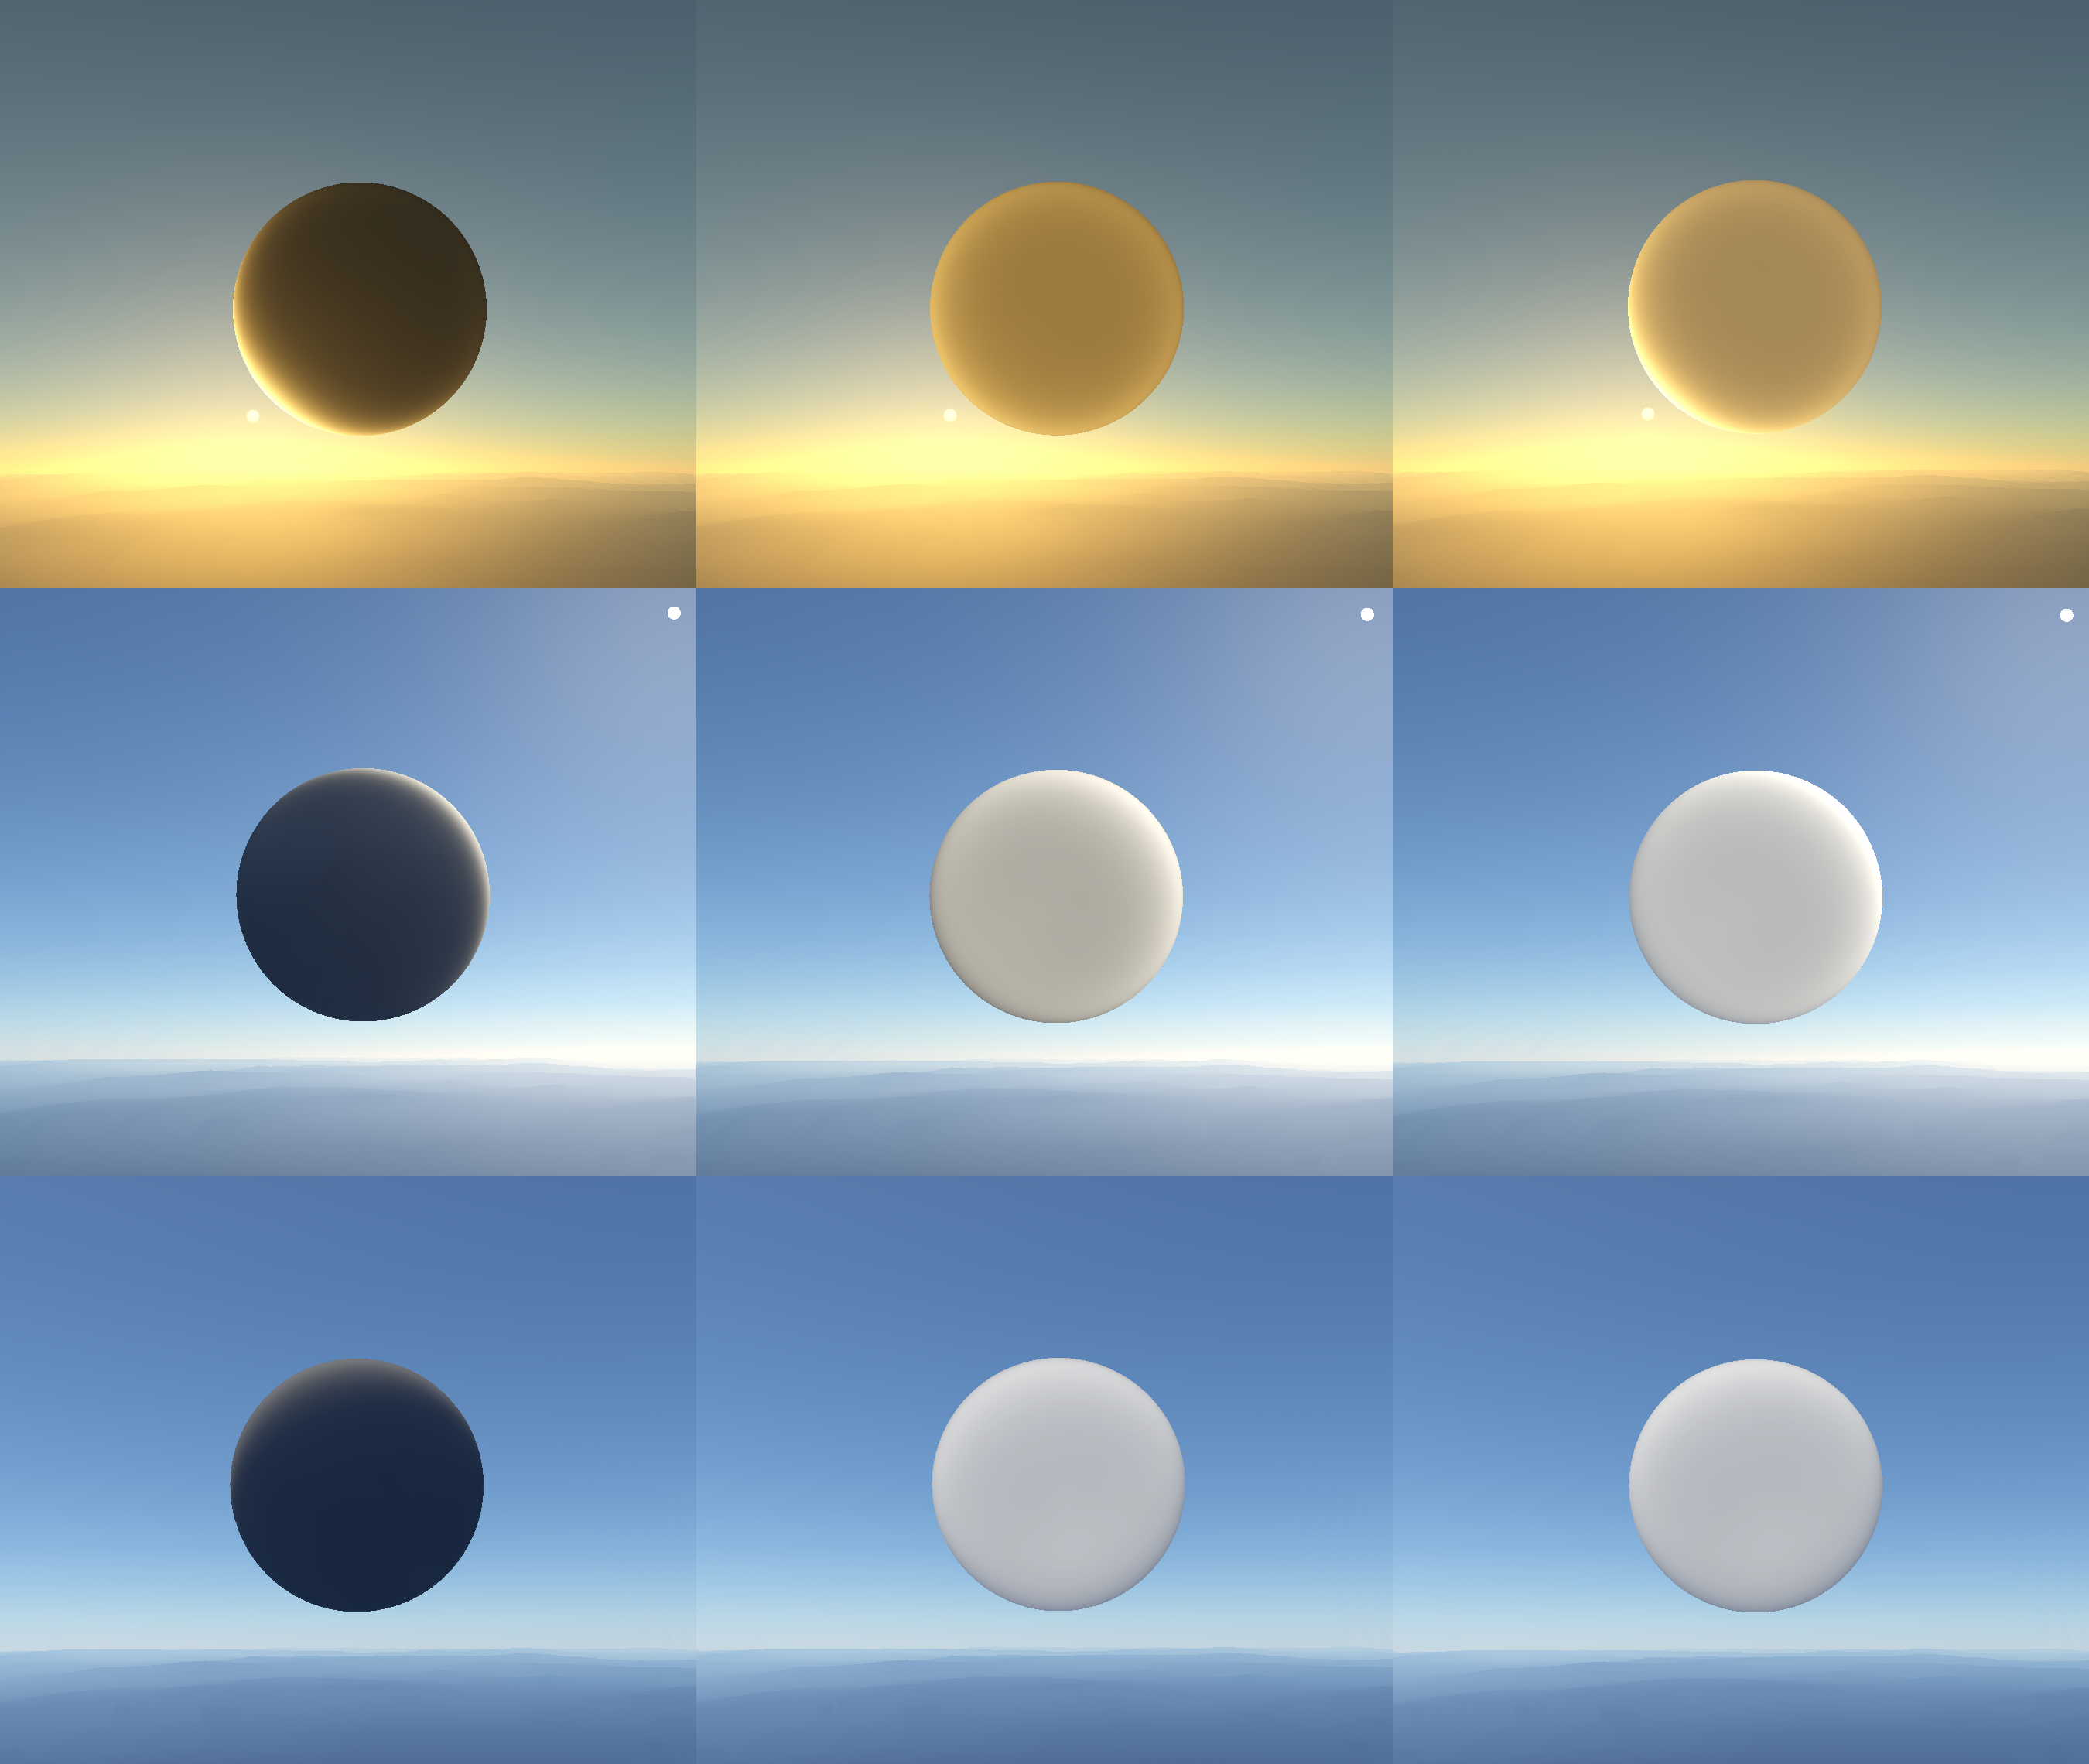
\includegraphics[scale=0.1]{images/scatteringresult.png}
\caption{Pre-computed scattering for different light orientations.
From left to right: single scattering only, 2 + scattering
only, all terms (including ambient). The particle in the bottom
row is illuminated from above}
\label{f12}
\end{center}
\end{figure}
\subsubsection{The Implementation}
We'll look into the implementation details of the 3 steps in this section.
\begin{enumerate}
\item Compute $\bar{J}^{(n)}$ for each point and direction inside the sphere.
\begin{lstlisting}
float GatherScatteringPS(SScreenSizeQuadVSOutput In) : SV_Target
{
    float4 f4LUTCoords = float4(ProjToUV(In.m_f2PosPS), g_GlobalCloudAttribs.f4Parameter.xy);

    float3 f3PosUSSpace, f3ViewRayUSSpace, f3LightDirUSSpace;
    ParticleScatteringLUTToWorldParams(f4LUTCoords, f3PosUSSpace, f3ViewRayUSSpace, f3LightDirUSSpace, false);

    float3 f3LocalX, f3LocalY, f3LocalZ;
    ConstructLocalFrameXYZ(-normalize(f3PosUSSpace), f3LightDirUSSpace, f3LocalX, f3LocalY, f3LocalZ);

    float fGatheredScattering = 0;
    float fTotalSolidAngle = 0;
    const float fNumZenithAngles = VOL_SCATTERING_IN_PARTICLE_LUT_DIM.z;
    const float fNumAzimuthAngles = VOL_SCATTERING_IN_PARTICLE_LUT_DIM.y;
    const float fZenithSpan = PI;
    const float fAzimuthSpan = 2*PI;
    for(float ZenithAngleNum = 0.5; ZenithAngleNum < fNumZenithAngles; ++ZenithAngleNum)
        for(float AzimuthAngleNum = 0.5; AzimuthAngleNum < fNumAzimuthAngles; ++AzimuthAngleNum)
        {
            float ZenithAngle = ZenithAngleNum/fNumZenithAngles * fZenithSpan;
            float AzimuthAngle = (AzimuthAngleNum/fNumAzimuthAngles - 0.5) * fAzimuthSpan;
            float3 f3CurrDir = GetDirectionInLocalFrameXYZ(f3LocalX, f3LocalY, f3LocalZ, ZenithAngle, AzimuthAngle);
            float4 f4CurrDirLUTCoords = WorldParamsToParticleScatteringLUT(f3PosUSSpace, f3CurrDir, f3LightDirUSSpace, false);
            float fCurrDirScattering = 0;
            SAMPLE_4D_LUT(g_tex3DPrevSctrOrder, VOL_SCATTERING_IN_PARTICLE_LUT_DIM, f4CurrDirLUTCoords, 0, fCurrDirScattering);
            if( g_GlobalCloudAttribs.f4Parameter.w == 1 )
            {
                fCurrDirScattering *= HGPhaseFunc( dot(-f3CurrDir, f3LightDirUSSpace) );
            }
            fCurrDirScattering *= HGPhaseFunc( dot(f3CurrDir, f3ViewRayUSSpace), 0.7 );

            float fdZenithAngle = fZenithSpan / fNumZenithAngles;
            float fdAzimuthAngle = fAzimuthSpan / fNumAzimuthAngles * sin(ZenithAngle);
            float fDiffSolidAngle = fdZenithAngle * fdAzimuthAngle;
            fTotalSolidAngle += fDiffSolidAngle;
            fGatheredScattering += fCurrDirScattering * fDiffSolidAngle;
        }
    
    // Total solid angle should be 4*PI. Renormalize to fix discretization issues
    fGatheredScattering *= 4*PI / fTotalSolidAngle;

    return fGatheredScattering;
}
\end{lstlisting}
Similarly, in this function \textbf{GatherScatteringPS}, the given projection position and the 4 parameters from the 4D look-up table is decomposed to 3 vec3 positions: the first one \textbf{f3PosUSSpace} describes the start position of the ray, the second one \textbf{f3ViewRayUSSpace} describes the ray direction, the last one \textbf{f3LightDirUSSpace} describes the light direction. Then we use the \textbf{zenith angles} $\varphi_v$ and \textbf{azimuth angles} $\theta_v$ count as the total steps, and we do the integration inside the two nested for loops. In each step, $\varphi_v$ and $\theta_v$ are increased by a step size. According to $\varphi_v$, $\theta_v$ and the start point, we calculate the ray direction \textbf{f3CurrDir}. After this, we transform the ray from world space back to the particle space. Then we check if the distance of the 4D table is 1 in order to calculate the current scattering direction \textbf{fCurrDirScattering} correctly. Finally, we accumulate the total scattering in each step by the amount of multiplying the current scattering direction \textbf{fCurrDirScattering} to the delta angle \textbf{fDiffSolidAngle}.\\
\textbf{SAMPLE\_4D\_LUT} is a utility function which returns an interpolated result into the 5th parameter from the first 4 parameters, which are 3D texture, Dim, coordinates and LOD index.


\item Compute $\bar{L}_{In}^{(n)}$ as the current order.
\begin{lstlisting}
float ComputeScatteringOrderPS(SScreenSizeQuadVSOutput In) : SV_Target
{
    float4 f4StartPointLUTCoords = float4(ProjToUV(In.m_f2PosPS), g_GlobalCloudAttribs.f4Parameter.xy);

    float3 f3PosUSSpace, f3ViewRayUSSpace, f3LightDirUSSpace;
    ParticleScatteringLUTToWorldParams(f4StartPointLUTCoords, f3PosUSSpace, f3ViewRayUSSpace, f3LightDirUSSpace, false);

    // Intersect view ray with the unit sphere:
    float2 f2RayIsecs;
    // f3NormalizedStartPos  is located exactly on the surface; slightly move start pos inside the sphere
    // to avoid precision issues
    float3 f3BiasedPos = f3PosUSSpace + f3ViewRayUSSpace*1e-4;
    GetRaySphereIntersection(f3BiasedPos, f3ViewRayUSSpace, 0, 1.f, f2RayIsecs);
    if( f2RayIsecs.y < f2RayIsecs.x )
        return 0;

    float3 f3EndPos = f3BiasedPos + f3ViewRayUSSpace * f2RayIsecs.y;
    float fNumSteps = max(VOL_SCATTERING_IN_PARTICLE_LUT_DIM.w*2, NUM_INTEGRATION_STEPS)*2;
    float3 f3Step = (f3EndPos - f3PosUSSpace) / fNumSteps;
    float fStepLen = length(f3Step);
    float fCloudMassToCamera = 0;
    float fParticleRadius = g_GlobalCloudAttribs.fReferenceParticleRadius;
    float fInscattering = 0;

    float fPrevGatheredSctr = 0;
    SAMPLE_4D_LUT(g_tex3DGatheredScattering, VOL_SCATTERING_IN_PARTICLE_LUT_DIM, f4StartPointLUTCoords, 0, fPrevGatheredSctr);
	// Light attenuation == 1
    for(float fStepNum=1; fStepNum <= fNumSteps; ++fStepNum)
    {
        float3 f3CurrPos = f3PosUSSpace + f3Step * fStepNum;

        fCloudMassToCamera += fStepLen * fParticleRadius;
        float fAttenuationToCamera = exp( -g_GlobalCloudAttribs.fAttenuationCoeff * fCloudMassToCamera );

        float4 f4CurrDirLUTCoords = WorldParamsToParticleScatteringLUT(f3CurrPos, f3ViewRayUSSpace, f3LightDirUSSpace, false);
        float fGatheredScattering = 0;
        SAMPLE_4D_LUT(g_tex3DGatheredScattering, VOL_SCATTERING_IN_PARTICLE_LUT_DIM, f4CurrDirLUTCoords, 0, fGatheredScattering);
        fGatheredScattering *= fAttenuationToCamera;

        fInscattering += (fGatheredScattering + fPrevGatheredSctr) /2;
        fPrevGatheredSctr = fGatheredScattering;
    }

    return fInscattering * fStepLen * fParticleRadius * g_GlobalCloudAttribs.fScatteringCoeff;
}
\end{lstlisting}

As always, firstly the function \textbf{ComputeScatteringOrderPS} computes the ray's start position, the direction, and the light direction. Again, moving the start point slightly inside the sphere to avoid precision issues. Then we calculate the intersected ray result, and step up some basic variables for the integration. We also calculate the interpolated result from the 3D texture of gathered scattering texture and store it into a variable called \textbf{fPrevGatheredSctr} as the initial scattering. In each integration step, we multiply the gathered scattering by the attenuation to the camera \textbf{fAttenuationToCamera}. Finally we accumulate the final scattering light into the camera \textbf{fInscattering} with the average amount of the scattering in this step \textbf{fGatheredScattering} and the scattering from the previous step \textbf{fPrevGatheredSctr}.

\item Accumulate current scattering order to the total look-up table: $\bar{L}_{In}^M = \bar{L}_{In}^M + \bar{L}_{In}^{(n)}$.
\begin{lstlisting}
float AccumulateMultipleScattering(SScreenSizeQuadVSOutput In) : SV_Target
{
    float3 f3LUTCoords = float3(ProjToUV(In.m_f2PosPS), g_GlobalCloudAttribs.f4Parameter.x);
    float fMultipleSctr = g_tex3DPrevSctrOrder.SampleLevel(samPointWrap, f3LUTCoords, 0);
    return fMultipleSctr;
}
\end{lstlisting}

This function \textbf{AccumulateMultipleScattering} is quite straightforward, it accumulates the multiple scattering.
\end{enumerate}

\section{Generating Real-time Shading Model}
